\todo{Introduction to section}
\section{List of model features and their biological foundation}

To write:
\begin{itemize}
    \item Table of parameters
    \item Shape of boundary condition

\end{itemize}
\subsection{Additions to the base model}
\note{Move to Appendix?}
\subsubsection{Improved simulation of apical constriction}
To emulate the lowering of apical surface area, invaginating cells ($\alpha > 0$) also got an increase in their $\lambda_1$'s making their relaxation distance shorter. This had the added benefit of echoing the tighter bonds in constricting cell clusters. [citation maybe needed]
\subsubsection{Cell types extracted from data}
When we say that the cell types were extracted from data, this comes with a couple asterisks:\\
Any expression in the cephalic region was removed by hand.\\
The second and third 
In the data-set there were no [Cephalic furrow gene], but using the website [website] we could see that it spatially coincided with [other gene] which was in the data-set and was therefore used as a proxy. 

\subsubsection{Ventral furrow}
While all cells expressing \textit{twist} \& \textit{snail} lower their apical surface area, they do not constrict indiscriminately, instead starting with the \textit{inner} 8x60 cells. [citation needed] It is believed to be a more stable way of wedging [citation needed] but is still strange and not fully understood. [citation needed]. This meant that a specific rule for the wedging in the ventral region was needed.

\subsubsection{Differential adhesion}
\subsubsection{Nematic $S_2$ and $S_3$}


\section{Visual closeness}
While the Drosophila embryo has been studied for decades, it is only relatively recently computer vision has gotten to a point where quantitative analyses of the more than 5000 cells has turned feasible. Therefore, like most of the fields history, we will start with examining the visual agreement between the morphology of simulation and data.

On the following page, our best in silico model and corresponding frames from [Stas' group] can be seen and compared:

\newpage

\begin{figure}[H]
    \centering
    \vspace*{-1cm}\hspace*{-1cm}\makebox[\textwidth]{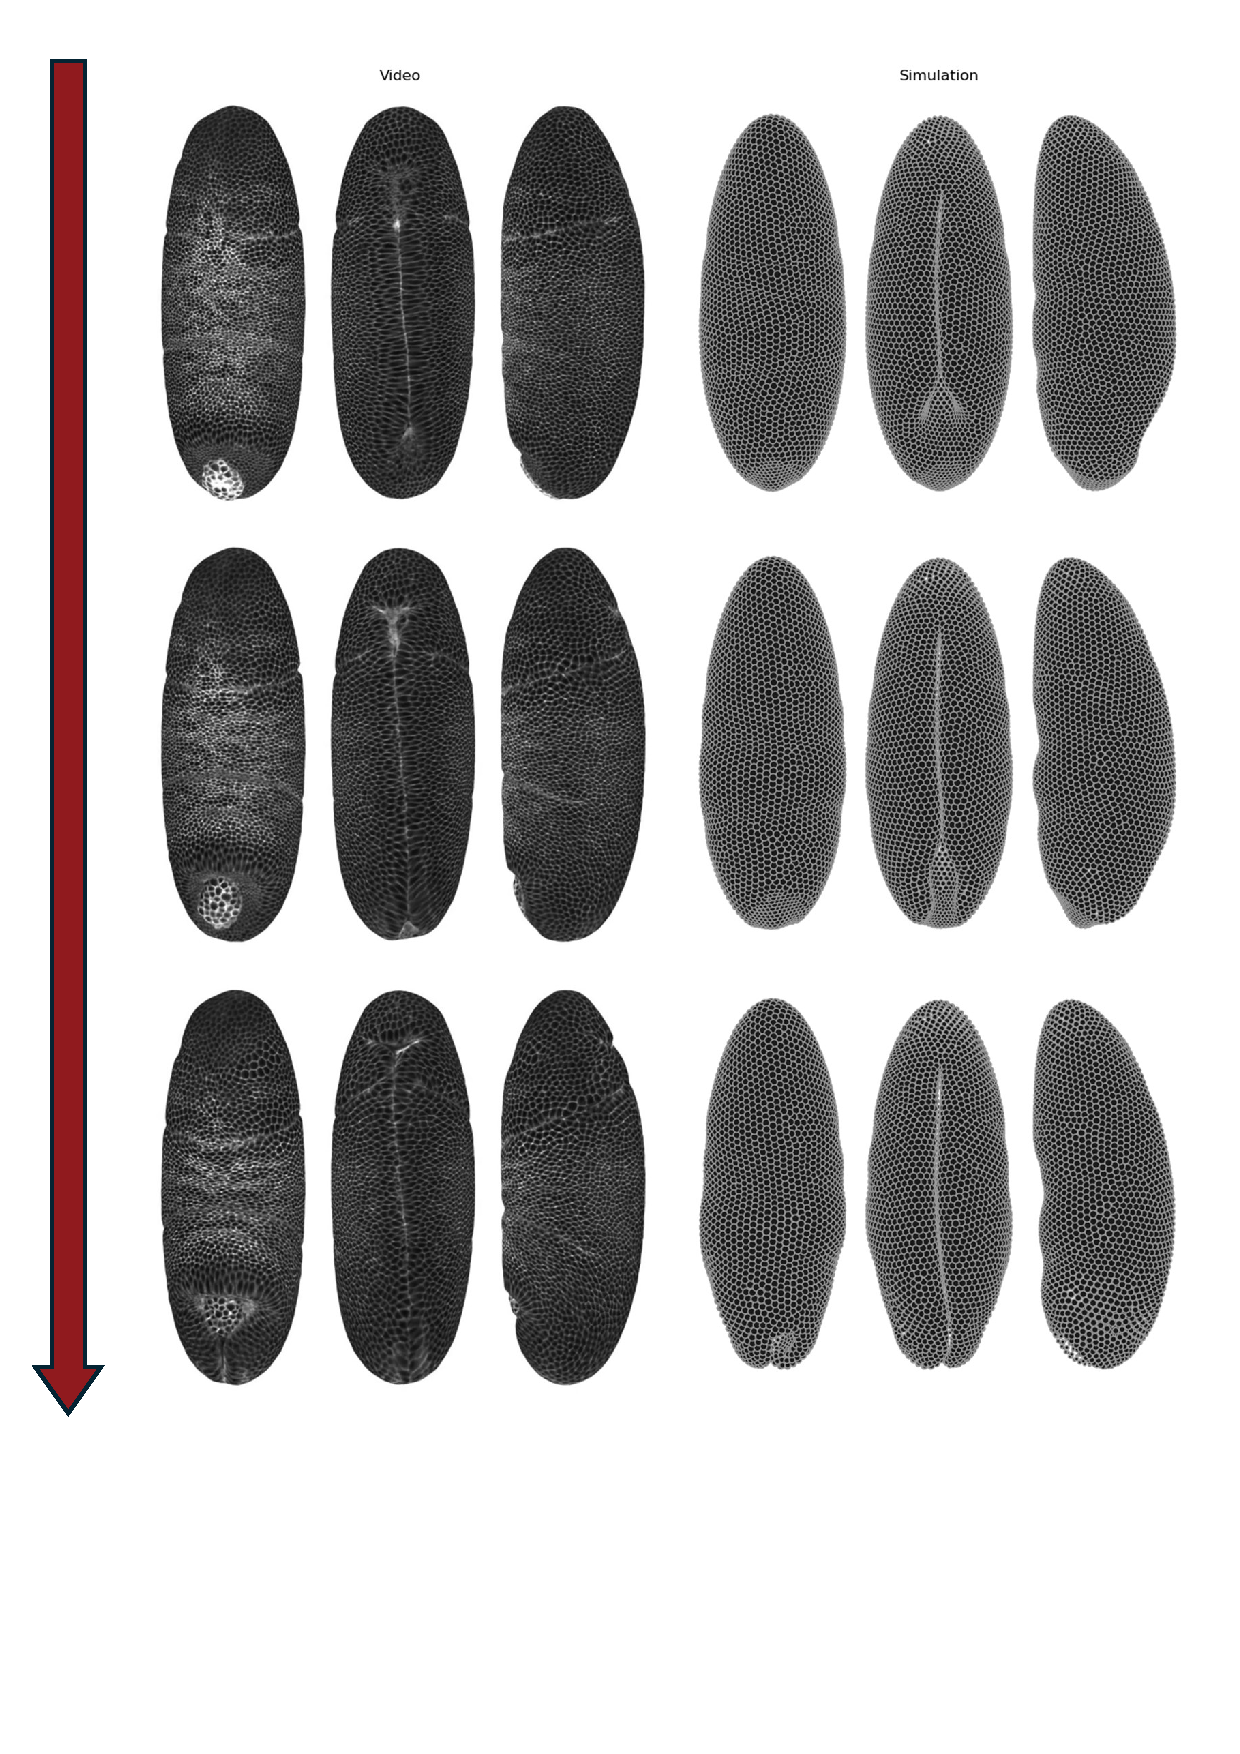
\includegraphics[width=0.85\paperwidth]{chapters/Results/figures/compare_to_vid_timeline.pdf}}
    \caption{Caption on next page}
    \label{fig:big-visual-comparison}
\end{figure}
\newpage
\addtocounter{figure}{-1}
\begin{figure} [t!]
  \caption{(Previous page.) \\A full page visual comparison between three timesteps of the simulation and in vivo imaging. For a more granular understanding this can be viewed in conjunction with Figure \ref{fig:big-timeline}.\\
  Each row consists of a single time-step. \textbf{Left:} In vivo. \textbf{Right:} In silico.\\Within each row, the embryo is show from the top (dorsally), bottom (ventrally) and laterally, with the posterior end pointing downwards.
  }
\end{figure}

Comparing, we can see that from a naïve inspection, not only has the general shape, timing and YYY been recapitulated, but YYY.  Given the relatively simple model and few specific alterations, this already seems impressive \note{maybe be more humble}, but to completely understand the agreements between data and simulation we will need to scrutinize the individual pieces using some visual aids. These will follow, but if you are ever YYYY, please return to Figure \ref{fig:big-visual-comparison} to get reminded of the big picture. 

\subsection{Ventral Furrow}
After mitosis stops, the the first visual change is on the belly where a distinct cleft begins forming. \\
As the furrow closes, it forms a closed-off tube with a recognizable light bulb-shape in the cross section. After closing YYY, the tube extends dorsally. This is the first building block [something] for the tubes that will become the gastrointestinal tract.

In figure \ref{fig:VFComparison}, a comparison between a cross section of our simulation and in vivo imaging can be seen.

\begin{figure}[H]
    \centering
    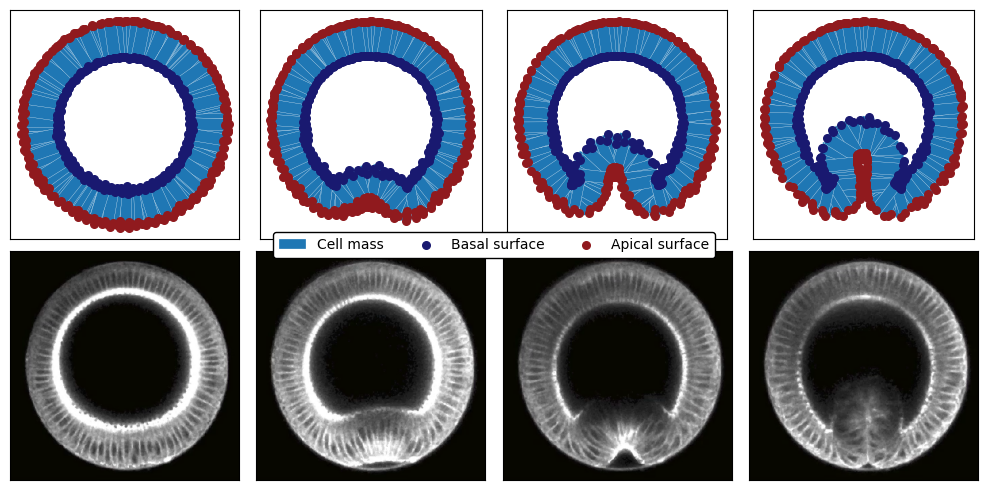
\includegraphics[width=1\linewidth]{chapters/Results/figures/VF_comparison.png}
    \caption{A comparison of simulation and frames from video of live growth. \\\textbf{Upper row}: Simulation. \textbf{Lower row}: Multi-photon microscopy. \\For ease of visualisation, each cell in the simulation is displayed as a rectangle along its AB-axis. Each frame is taken at equally spaced time intervals. Cross section video borrowed from \cite{conte2012biomechanical}}
    \label{fig:VFComparison}
\end{figure}


Our simulation extends slightly more [upwards] (this is especially noticable closer to the anterior tip), but in general, the formation of the ventral furrow has been ...

\todo{Maybe quantify here?}\\
I am guessing we can do a cell-center fit?
Is this out of scope? Yes. Would it be cool? Also yes.
\subsection{Germ band}
The largest [something] on the blastoderm is the Germ Band which fills most of the lateral sides. As mentioned in Section \ref{sec:drosophila-embryo-detail}, it is generally agreed that the Germ Band is one of the main drivers of anterior-posterior motion (although it remains disputed how).

In Figure \ref{fig:germbandCompare} a text-book diagram of the motion of the Germ Band can be compared with the shape of the Germ Band in the first and last frame of our simulation. 

\begin{figure}[H]
    \centering
    \begin{subfigure}[b]{0.34\textwidth}
        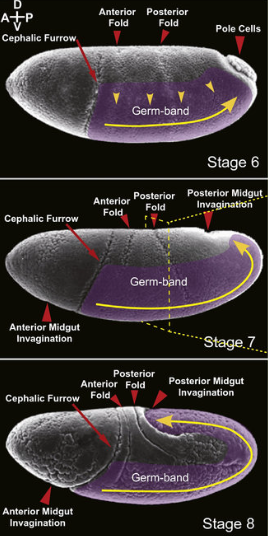
\includegraphics[width=\textwidth]{chapters/Results/figures/compareGB.png}
    \caption{Figure taken from \cite{kong2017forces} }
    \end{subfigure}
     \hfill
    \begin{subfigure}[b]{0.61\textwidth}
    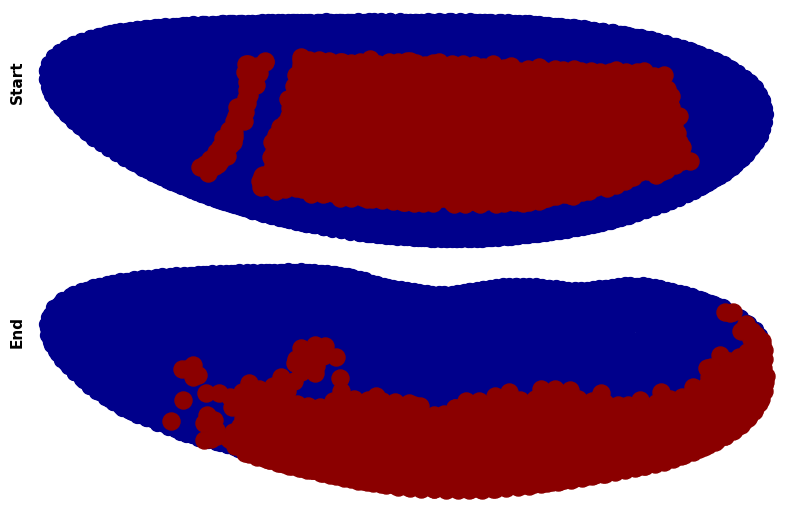
\includegraphics[width=\textwidth]{chapters/Results/figures/gb_firstframe_lastframe.png}
    \caption{Simulation with colored in Germ Band}
    \end{subfigure}
    \caption{A visual comparison between a diagram of the Germ Band cells and the cells as defined in our simulation\\Note: The blue line separating the Germ Band in the initial frame is a quirk of the gene-expression-cutoff as described in Section \ref{sec:drosophila-embryo-detail}.}
    \label{fig:germbandCompare}
\end{figure}


In general we see a great agreement in the morphological timeline of the Germ Band between simulation and data. Both the migration ventrally and "wrapping around" at the posterior tip. For a representation of the motion of individual cells, see Figure \ref{fig:GBMovements} in the Appendix.


\subsection{General morphology}
In the literature, a common way of visualizing the changes in both local and global structure, consist of (virtually) drawing in straight lines on the [fly] at the onset of gastrulation and seeing how they translate and skew over time. An example in both data and simulation can be seen in Figure \ref{fig:band-movements-stas}.

\begin{figure}[H]
    \centering
    \makebox[\textwidth][c]{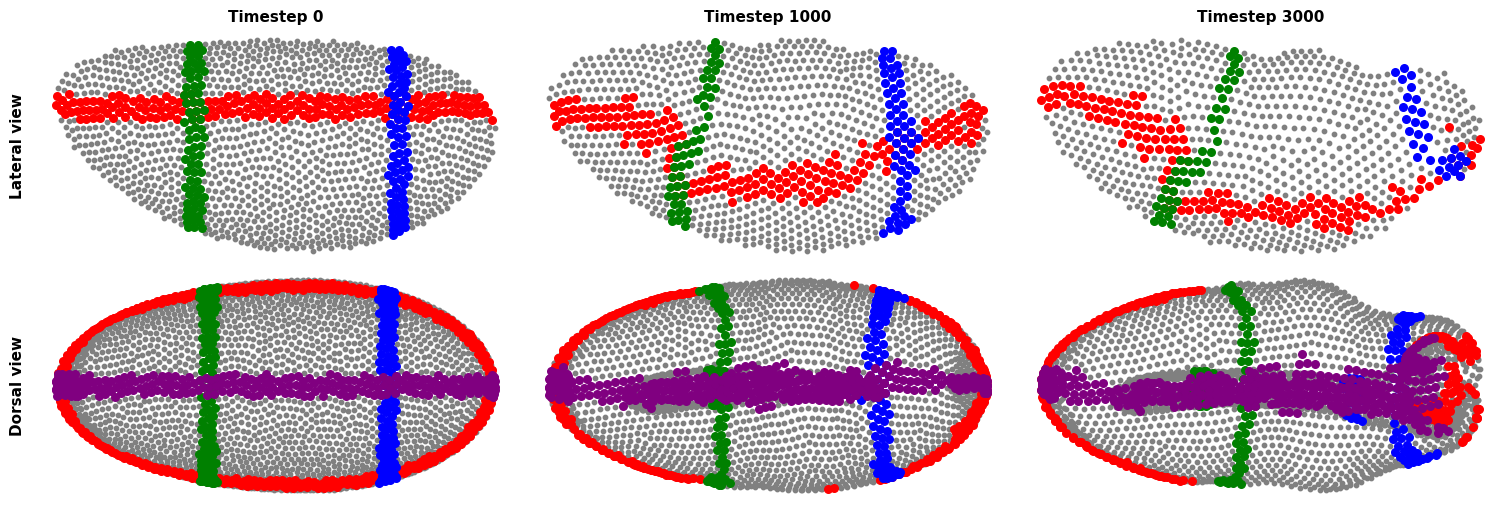
\includegraphics[width=1.1\linewidth]{chapters/Results/figures/band_movements.png}}
    % \caption{My simulation. Compare to figure \ref{fig:band-movements-stas}}
    % \label{fig:band-movements}
\end{figure}
\begin{figure}[H]
    \centering
    \makebox[\textwidth][c]{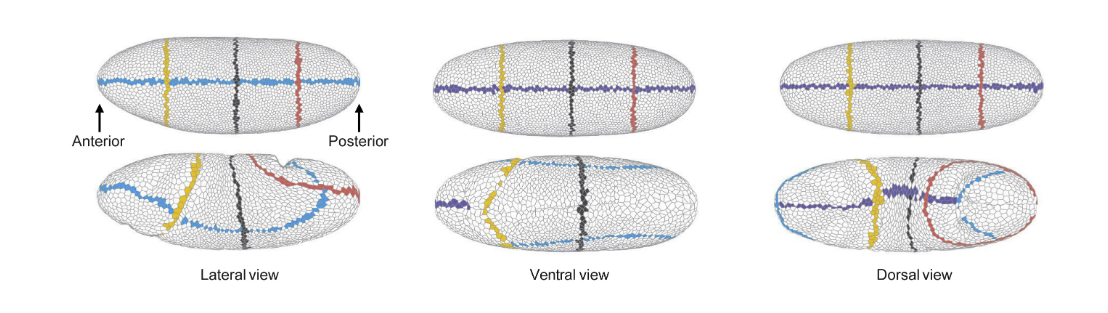
\includegraphics[width=1.\linewidth]{chapters/Results/figures/compareStasGBShape.png}}
    \caption{Position of specific bands over time.\\ \textbf{Top row:} Simulation | \textbf{Bottom row:}  Segmented images (from \cite{stern2022deconstructing}). \\\todo{make colors match.}}
    \label{fig:band-movements-stas}
\end{figure}

This juxtaposition/contrast allows for some interesting observations:\\
As is evident, there is a general agreement between both local and large-scale changes in embryonic form. 

The posterior tip has some trouble where cells "fall out of line" nd the line becomes muddled.

Where the cephalic furrow is supposed to be (green vertical line), the epithelial sheet has less wiggle room in simulation than what is needed and also struggles to move "smoothly".\note{too jovial} 

The simulation is not [stable] for a as much motion anteriorly as we see IRL





\subsection{Daniel}
\todo{Make use of section or cut}
\section{Quantitative closeness}
While comparing the motions/morphogenesis visually is interesting, we are physicists and would like some quantification of the model performance.

It was stated earlier that [hard] data is tough to come by. \footnote{We have even been in contact with a guy who spent a large amount of his PHD to simply hand-track a single 20 cell band in 3 embryos} But recent technical advancements in microscopy and computational cell-segmentation has given rise to the possibility of large-scale automated [statistically significant] analyses. 
\subsection{Movements}

Our interests lie in the [BC IC], but the system is . To 

As we have no way of doing any one-to-one cell comparisons, and [what we are after is large scale kinetics], the following measure was devised: 

For ever n'th time-step, look at the recent motion of each cell. Compare each of these to the average motion vector of the 10 spatially closest cells in data. 


The resulting angle difference between 0 and $\pi$ is scaled to be between 0 and 1, with 1 being perfect agreement.

\begin{figure}[H]
    \centering
    \makebox[\textwidth][c]{
    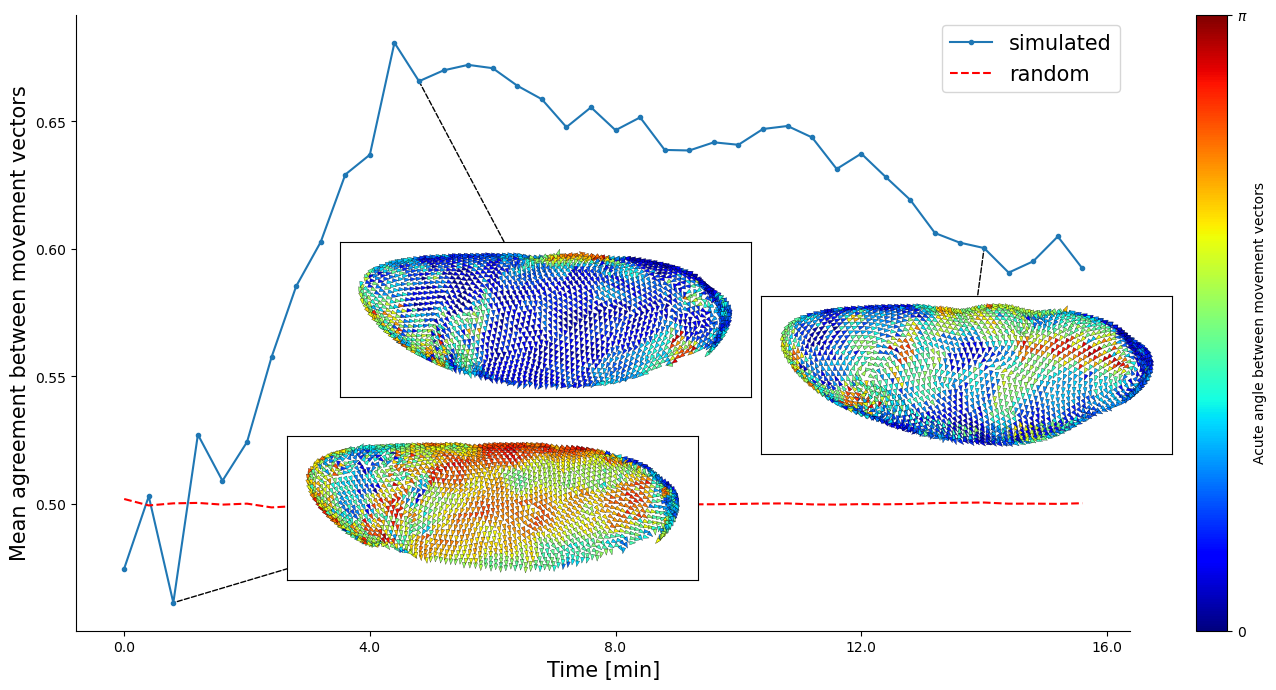
\includegraphics[width=1.3\linewidth]{chapters/Results/figures/movement_vectors_normal.png}
    }
    \caption{The motion-vector agreement across the full embryo of the single (visually) best run as a function of time\\
    The red \textit{random}-line is a simulated embryo where every direction is uniformly randomly chosen. \todo{fix x-axis}}
    \label{fig:motionAgreement}
\end{figure}

Figure \ref{fig:motionAgreement} gives us quantitative confidence that, not only does the whole morphogenesis follow the general YYY, but the individual [atoms] also align with the.

It is very clear that in the first two minutes our simulation and reality does not agree. 



In general, we see a consistent, well-above average overlap. 

I'd like to stress the fact, that having the individual atoms align with the average motion of other. Convergent extension is by its very nature based on the global motion being being more important than the individual (see figure \ref{}) 

To combat this even

Looking how the error is distributed:
\begin{figure}[H]
    \centering
    \makebox[\textwidth][c]{
    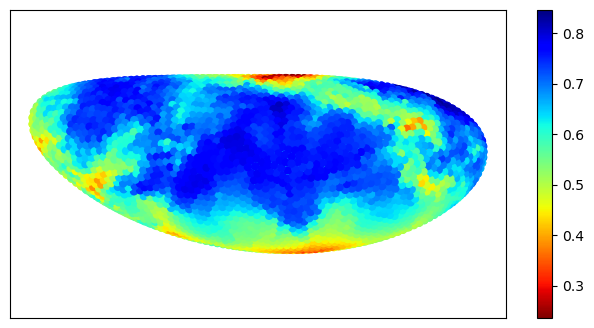
\includegraphics[width=0.8\linewidth]{chapters/Results/figures/movement_mapped_normal.png}}
    \caption{The motion-vector agreement across the full run mapped back onto their original positions \todo{colorbar label}}
    \label{fig:motionAgreement}
\end{figure}


Important to note:
he data consist of machine-tracked cell positions. This means any radial motion is neglected.
If we take into account that the original data only supported motion-tracking on the visible exterior surface, it makes sense that the whole 8x60 cell early invaginating Ventral region is YY no agreement. 

Also dorsal folds

Even though the a lot of the leftmost (anterior) part of the embryo is mostly still until cephalogenesis sets in, the head-tissue primordium has been deemed outside of scope of the current project.

This gives us the idea to only looking at the dynamical parts of the egg:

\begin{figure}[H]
    \centering
    \makebox[\textwidth][c]{
    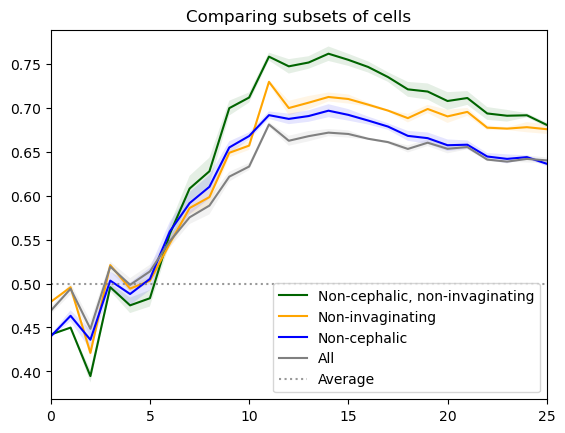
\includegraphics[width=1\linewidth]{chapters/Results/figures/movement_vectors_normal_subsets.png}
    }
    \caption{The motion-vector agreement across the full embryo as a function of time. For confidence is the stability of the current solution, all lines and shaded areas are averages and and standard deviations of three runs using identical parameters but different seeds.}
    \label{fig:motionAgreement}
\end{figure}

Focusing on the parts of the [embryo] we have a chance to [recapitulate] we get an almost 80 percent average agreement.  

Conclude


\subsection{Timing}
Cells have been shown to have remarkably precise internal clocks\footnote{cool footnote with a remarkable number\cite{cellinternal}} and chemical gradients in the embryo changing across timescales from seconds to hours\cite{shvartsman2008dynamics}. There is also the "biological clock"\cite{johanolsen2} that proteins themselves have dynamic structure that can change over time.\cite{johanolsen1}. But there is no evidence for any specific timing in stages 5-7 [citation needed]. We would like to stress the importance of the result our model seem have recapitulated much of the dynamics completely without any explicit time-dependent parameters. This could be seen to corroborate the fact that Boundary Conditions, Initial Conditions and an inter-atomic rule-set is sufficient for some of the complex morphology/anatomy to arise. 


\subsection{Strain}
As the tissue warps and skews the cells are both subject to- and drivers of- stress and strain on the cell walls. This is one of the most widely studied parts of structural changes in morphogenesis.

While our simulation neither includes cell walls nor explicit strain calculation, computer-vision method has been developed which we can utilize. The Green-Lagrangre algorithm, as utilized in \cite{butler2009cell} for example, looks at local deformations in the tissue\footnote{The algorithm and implementation is written out in Section \ref{App:Strain-Calculation} in the Appendix}. In figure \ref{fig:strain} the results of an implementation can be seen and compared to a implementation run on software-segmented image.

\begin{figure}[H]
    \centering
    \begin{subfigure}{0.45\linewidth}
        \centering
        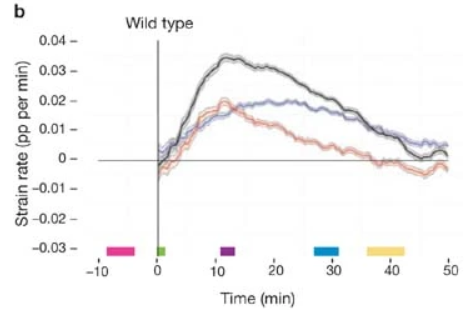
\includegraphics[width = \linewidth]{chapters/Results/figures/strain_rate_extrinsic.png}
    \end{subfigure}
        \begin{subfigure}{0.45\linewidth}
        \centering
        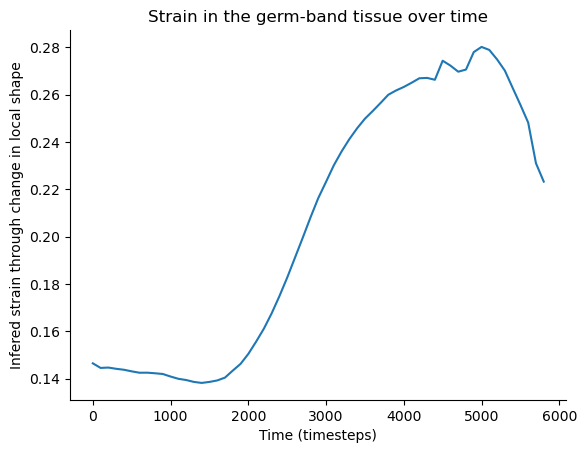
\includegraphics[width = \linewidth]{chapters/Results/figures/strain_smoothedpng.png}
    \end{subfigure}
    \caption{Comparison between Figure 1 from \cite{butler2009cell}. And an implementation of their strain-inference algorithm. Quick rise followed by a fall-off at time of PMG invagination\\\todo{Explain the leftmost plot or find another that shows the same with only one line}}
    \label{fig:strain}
\end{figure}



It can be seen in the first 12-15-minutes which we are, we see a rising strain, ending at the point of internalization of the germ cells ($\approx12$minutes). In our simulation, the strain has a delayed onset. The fact that the first 2 minutes have a central difference from ground truth is a recurring theme.

Conclude\\

Tie into next

\subsection{Rosettes}
As Convergent Extension is said to be one of the main contributors for epithelial cell motility, a lot of analyses have been developed. \todo{I must have been tired when I wrote this. Rephrase!}
One of the main quantifiers 

When looking at a cluster of cells that undergo convergent extension. Their protein-tendrils can be far reaching. Trough laser-ablation is has been shown that Rosettes (as shown in the diagram on Figure \ref{fig:ConvergentExtensionDiagram}) can be up to twelve [citation needed].
For drosophila gastrulation in particular, the direction between each newly acquired neighbor.



% \begin{figure}[H]
%     \centering
%     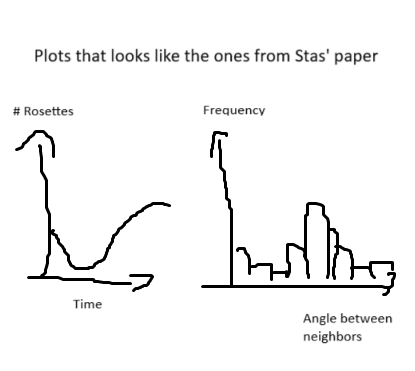
\includegraphics[width=0.8\linewidth]{chapters/Results/figures/rosettes_placeholder.png}
%     \caption{Caption}
%     \label{fig:enter-label}
% \end{figure}

In Figure \ref{fig:roestte-angle-dist}, the distribution of angles of all found rosette-events can be seen. Strangely, the distribution is clearly bimodal, where the ground truth has a single peak.

\begin{figure}[H]
    \centering
    \makebox[\textwidth][c]{
    \begin{subfigure}[b]{0.55\textwidth}
    \centering
        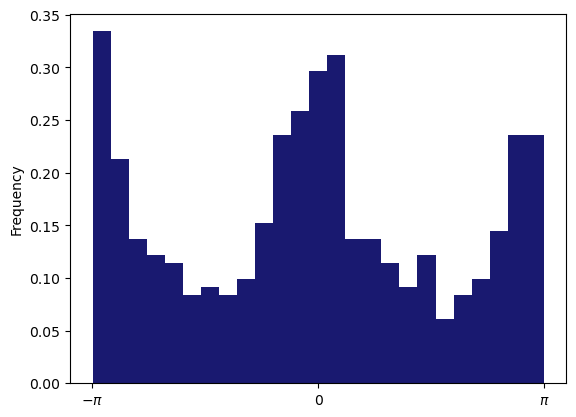
\includegraphics[width=\linewidth]{chapters/Results/figures/rosettes_angle_dist.png}

    \end{subfigure}
    \begin{subfigure}[b]{0.5\textwidth}
    \centering
    
    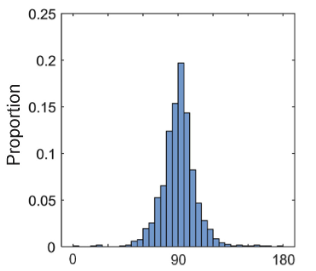
\includegraphics[width=\linewidth]{chapters/Results/figures/rosettes_angle_dist_data.png}
    \end{subfigure}
    }
    \caption{The angular distribution of the newly acquired neighbors in rosettes as found in (\textbf{left}) simulation (in radians) and (\textbf{right}) data (in degrees).}
    \label{fig:roestte-angle-dist}
    
\end{figure}


When speaking with Daniel, a researcher at the [Stas'] laboratory who did the original analysis, he said that this makes sense, as looking at neighboring nuclei is fundamentally different from edges. \todo{rephrase to make less bad}. 

I won't bore you the details, so a quick run-down of our thoughts and discussions can be found in Section \ref{App:why-rosettes} in the Appendix.\\

... \\
Speaking of Daniel:


\subsection{Daniel-data?}
Nothing here yet, Ala. But I am hopeful!
\begin{figure}[H]
    \centering
    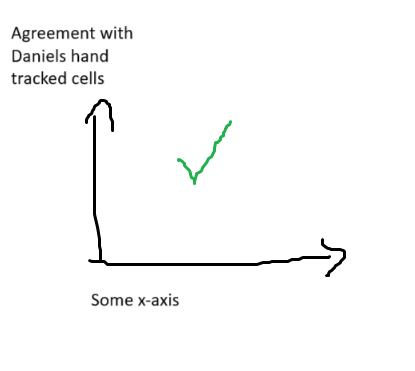
\includegraphics[width=0.7\linewidth]{chapters/Results/figures/daniel_placeholder.png}
    \caption{Some caption}
    \label{fig:enter-label}
\end{figure}
\newpage
\section{In Silico Mutant "predictions" - compared to phenotypes and reference model}
Having a complete simulated [pipeline] from (simplified) morphogen to (approximate) morphogenesis, opens the door for some intriguing explorations into our model and its relation to nature.\\

A large branch of developmental biology experiments consists of discovering or creating genotypes, and cataloging the resulting organisms. The genetic markup of animals that are deficient in some YYY. 
Our model allows for the creation of genetically-variant, by changing the response to one or more of the simulated morphogens.\\


\subsection{No PMG}
In [cite Stas] and [cite Stas again], they show that the chemical signals produced by the protein \textit{Hkb} are initiates the formation of the midgut by wavelike patterns of isotropic apical constriction around the posterior tip. In \textit{Hkb}-deficient mutants the lack of posterior invagination has a clear response. The build up pressure from the extending germ-band causes the . This has given the \textit{Hkb}-mutant the nickname "corkscrew mutant"\footnote{Timmy Glenn}.\\

In Figure \ref{fig:corkscrew-comparison}, a video of the corkscrew mutant can be compared to our simulation after removing the cells ability to react to \textit{Hkb}.

 
\begin{figure}[H]
    \centering
    \makebox[\textwidth][c]{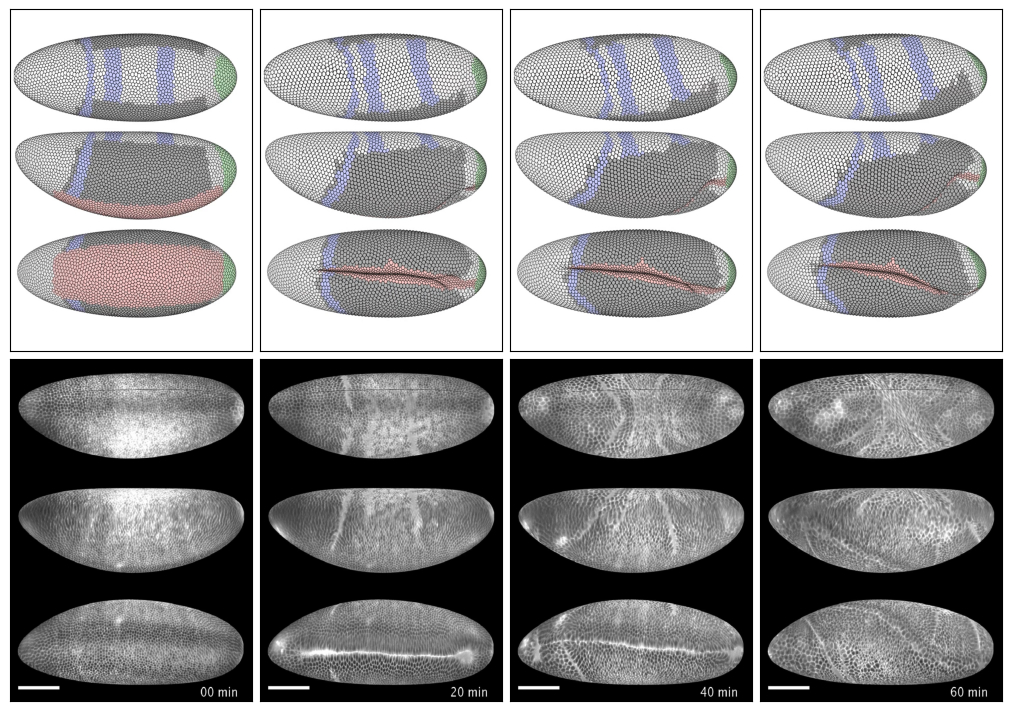
\includegraphics[width=1.2\linewidth]{chapters/Results/figures/corkscrew_comparison.png}}
    \caption{Comparing the \textit{Corkscrew} phenotype with my simulation. Video taken from \cite{smits2023maintaining}.}
    \label{fig:corkscrew-comparison}
\end{figure}
% Twist and shout

Comparing the reaction of these In Silico Mutants to real life phenotypes gives us a hint of capturing more than we we put in. TODO: make sound good. 

\subsection{No Ventral Furrow}
When knocking out the \textit{Twist} and \textit{Snail} genes, which, as you might remember, are primary organizers of apical constriction, the ventral furrow fails to form. 
% \url{https://genesdev.cshlp.org/content/5/9/1568.full.pdf}
% We are seeing the right thing
We are seeing the right thing.


\subsection{Auxiliary(cephalic furrows}

In the absence of controlled folding of the dorsal tissue, the pressure from the extending Germ Band, can lead to other folds(?) \url{https://brunovellutini.com/posts/cephalic-furrow-thread/}

This is key to both understanding why the invaginated posterior end does not travel further anteriorly.

Also the large scale morphology change some runs had.

\subsection{No active intercolation / Germ band}
\label{sec:mutantNoGB}
We know that \textit{Runt} and \textit{Even skipped} are upstream . The litterature is conflicted, but the general theory is, that the patterning allows for a coherent orientation of the planar cell polarity. 

PCP-orientation was set at the intial step of the simulation as pointing in the distinct direction defined by the interspersed \textit{Runt} and \textit{Even skipped} patterning.
The results are interesting, albeit very uneventful, as
In the litterature  \cite{butler2009cell} more the morphogenesis is driven by more than Convergent Extension, and unstriped mutants are still viable, unlike our case where nothing happens.

Seems to be a clear indicator for active cell shape change being a vital part of... 

TODO: Discuss level of abstraction in the model 

\section{Combining and comparing to each other}
Given that we have a world-first [citation needed] full embryo model, Even with its flaws, in silico experiments about how the different dynamical parts of the embryo interacts can be very interesting. \todo{omformulér}

We will be doing it, both by comparing the different 'phenotypes' to our baseline model, i.e. seeing how important the cell types are for a gastrulation that is comparable to the current best.

We introduce the metric \textit{Pole Cell Migration} as a virtual metric for the success of the gastrulation. The Pole Cell Migration is defined as the percentual angle change of the posterior tip in the lateral plane \todo{make figure? or just explain better}. As we have seen, the slow start followed by a sudden push seems to be a defining characteristic for the gastrulation. In Figure \ref{fig:PCM-mutants} a comparison of multiple runs of the "simple" mutants. \note{maybe no need to introduce PCM as a shorthand}

\begin{figure}[H]
    \centering
    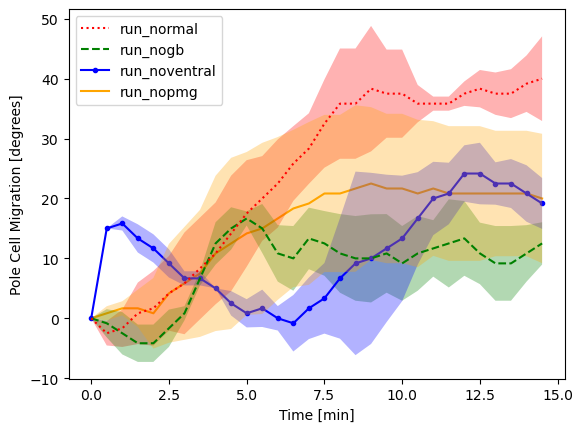
\includegraphics[width=1.\linewidth]{chapters/Results/figures/compare_PCM.png}
    \caption{\todo{Explain, fix x-axis}}
    \label{fig:PCM-mutants}
\end{figure}

Videos of the individual runs can be found in Section \ref{App:videos} in the Appendix, but a lot of the dynamics of the system can be gathered from the motion of the posterior tip. We can se that:\\
\textbf{Normal (red):} \\
\textbf{No Germband (green):} Without the pressure form the actively expanding germband, the motion purely from the invaginations. As the ventral cells also had $\lambda_3>0$ the there is still a tendency to move the tip dorsally, but there is not enough force for the posterior tip to move away from the [krængende]\todo{Translate} end of the egg allowing for the iconic [indfold]. \\
\textbf{No Ventral Furrow (blue):} Firstly, when no tissue is pulled into the ventral side, the extending germband allows for an upwards push to the germband. This is negated, as we remove the VF-cells from the equation, the germ-band is not moved ventrally. This means they exert their pressure uniformly from the port and starboard sides not translating.\\
\textbf{No PMG (yellow):} Here we see a possible breakdown of this metric, as, just like the in vivo experiments has show, the posterior tip moves slightly . None of the corkscrew-twising is captured. Not knowing how bad  50\% too little pole cell migration is, it does not capture just how unviable an embryo with this mutation is.   \\
\todo{This is very jovial, rewrite but keep same points.}\\


Now for a more granular approach, we boil the PCM down to a single number quantifying the total dorsal motion. In the matrix in Figure \ref{fig:PCM-matrix} we have calculated\footnote{emitting about 7kg of CO2 \url{https://mlco2.github.io/impact} } the combined effects of missing any two can be seen. 

\begin{figure}[H]
    \centering
    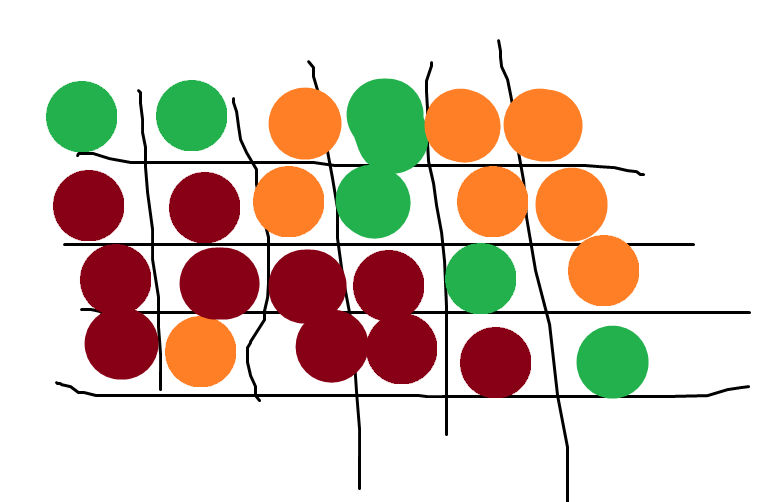
\includegraphics[width=1.\linewidth]{chapters/Results/figures/placeholder_domain_matrix.png}
    \caption{Caption}
    \label{fig:PCM-matrix}
\end{figure}

\todo{Find something interesting to discuss}

\section{Combining and comparing to data}
While comparing internally is interesting and can say a lot about the dynamics, we wanted a short detour where we recreate Figure \ref{fig:motionAgreement}, seeing how each mutation changes the motion-vectors. The results can be seen in Figure \ref{fig:compare-motionAgreement} below.

\begin{figure}[H]
    \centering
    \makebox[\textwidth][c]{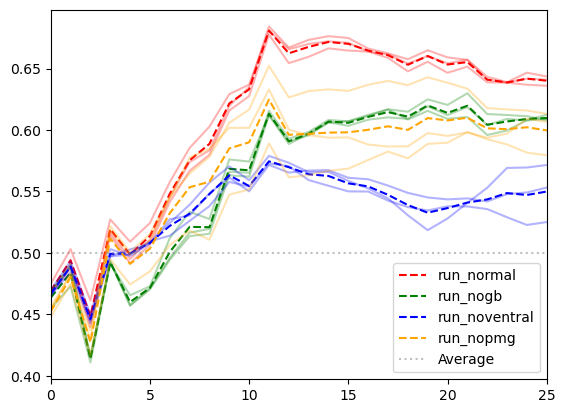
\includegraphics[width=1.3\linewidth]{chapters/Results/figures/PLACEHOLDER_compare_movement_vectors.png}}
    \caption{This is the main plot of the thesis. Y-axis is sum of y-axis of over all times in Figure \ref{fig:motionAgreement}. \todo{make better legend and axis labels}}
    \label{fig:compare-motionAgreement}
\end{figure}
It is comforting to see,
\todo{Find something interesting to discuss}

\begin{figure}[H]
    \centering
    \makebox[\textwidth][c]{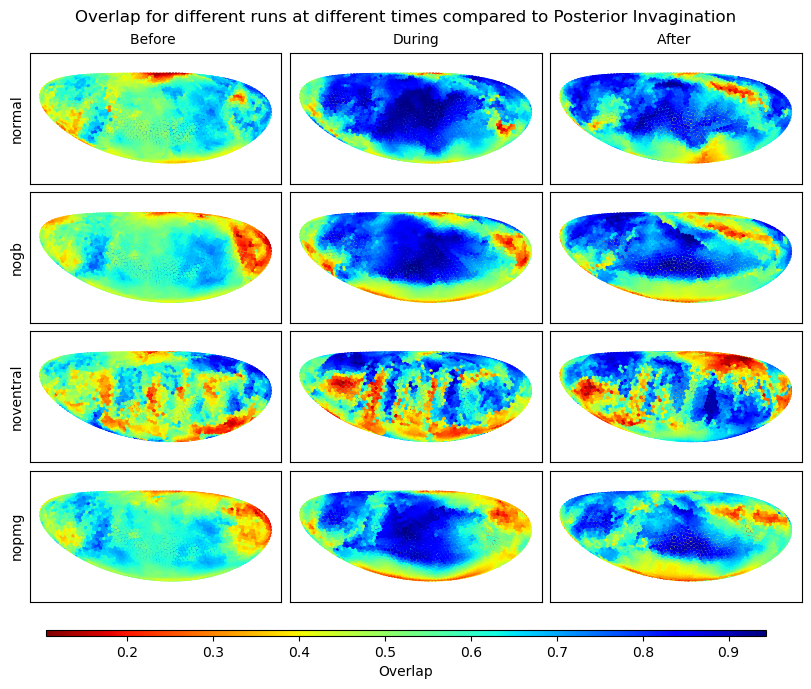
\includegraphics[width=1.3\linewidth]{chapters/Results/figures/Compare_all_movements.png}}
    % \caption{This is the main plot of the thesis. Y-axis is sum of y-axis of over all times in Figure \ref{fig:motionAgreement}}
    % \label{fig:compare-motionAgreement}
\end{figure}

\subsection{Without gene-defined PCP-initialization}

\section{Parameter Sensitivity Analysis}
No good YY of a simple model is complete without a Parameter Sensitivity Analysis.





% \url{https://softmath.seas.harvard.edu/wp-content/uploads/2019/10/2009-07.pdf}
% clear that model is missing cell shape change!
% \section{Additive/subtractive working together matrix}
% \subsubsection{}